% =============================================================================
%  Secao autonoma sobre o sensor de corrente (SS49E + nucleo toroidal)
%  Documento AUTOSSUFICIENTE (nao depende do projeto abntex2 da tese) -- feito
%  pra compilar sozinho com pdflatex e ser revisado aqui antes de ser
%  transplantado manualmente para o documento principal do TCC.
%
%  Compilar (quando houver pdflatex disponivel):
%      pdflatex SensorCorrente.tex
% =============================================================================
\documentclass[12pt,a4paper]{article}

\usepackage[utf8]{inputenc}
\usepackage[T1]{fontenc}
\usepackage[brazilian]{babel}
\usepackage{geometry}
\geometry{a4paper, margin=2.5cm}
\usepackage{graphicx}
\usepackage{amsmath}
\usepackage{siunitx}
\sisetup{output-decimal-marker = {,}, exponent-product = \cdot, tight-spacing=true, group-digits=false}
\usepackage{booktabs}
\usepackage{caption}
\usepackage[colorlinks=true, linkcolor=black, citecolor=black, urlcolor=black]{hyperref}
\usepackage{tikz}
\usetikzlibrary{decorations.pathmorphing, decorations.pathreplacing, arrows.meta}

\title{Sensor de Corrente: SS49E + Núcleo Toroidal\\
\large Rascunho de seção -- Metodologia/Resultados}
\author{}
\date{}

\begin{document}
\maketitle

\section{Sensor SS49E}
\label{sec:ss49e}

A medição de corrente de fase é realizada por um sensor Hall linear e
ratiométrico (SS49E): a tensão de saída varia linearmente com a densidade de
fluxo magnético ($B$) aplicada perpendicularmente ao elemento sensor, em
torno de um nível de repouso. O elemento é posicionado no entreferro de um
núcleo toroidal de ferrite que envolve o condutor de potência em uma única
espira, atuando como concentrador de fluxo: o caminho magnético de alta
permeabilidade intensifica, no entreferro, a densidade de fluxo produzida
pela corrente muito além do que se obteria com o sensor exposto diretamente
ao campo do condutor. A caracterização elétrica do próprio SS49E, extraída
do \textit{datasheet} do fabricante, está resumida na
Tabela~\ref{tab:datasheet_ss49e}.

\begin{table}[h]
\centering
\caption{Características elétricas do SS49E ($T_A = \SI{25}{\celsius}$, $V_{CC} = \SI{5,0}{\volt}$).}
\label{tab:datasheet_ss49e}
\begin{tabular}{lccccc}
\toprule
\textbf{Parâmetro} & \textbf{Símbolo} & \textbf{Mín.} & \textbf{Típ.} & \textbf{Máx.} & \textbf{Unidade} \\
\midrule
Tensão de alimentação (operação) & $V_{CC}$ & 3,0 & -- & 6,5 & V \\
Corrente de alimentação & $I_{CC}$ & -- & 4,2 & 8,0 & mA \\
Corrente de saída & $I_{OUT}$ & -- & 1,0 & 1,5 & mA \\
Tempo de resposta & $t_{ack}$ & -- & -- & 3 & \si{\micro\second} \\
Tensão de repouso ($B=0\,\text{G}$) & $V_O$ & 2,25 & 2,50 & 2,75 & V \\
Sensibilidade & $S_H$ & 2,0 & 2,5 & 3,0 & mV/G \\
Tensão mín. de saída ($B=\SI{-1500}{\gauss}$) & -- & -- & -- & 0,86 & V \\
Tensão máx. de saída ($B=\SI{+1500}{\gauss}$) & -- & -- & -- & 4,21 & V \\
Linearidade (\% do \textit{span}) & -- & -- & -- & 0,007 & \% \\
Erro de temperatura (\textit{null drift}) & -- & -0,10 & -- & 0,10 & \%/\si{\celsius} \\
Deriva de sensibilidade ($T_A \geq 25\si{\celsius}$) & -- & -0,15 & -- & 0,05 & \%/\si{\celsius} \\
Deriva de sensibilidade ($T_A < 25\si{\celsius}$) & -- & -0,04 & -- & 0,185 & \%/\si{\celsius} \\
\bottomrule
\end{tabular}

\vspace{2pt}
{\small Fonte: Autor (2026), a partir do \textit{datasheet} do fabricante.}
\end{table}

Dois pontos do \textit{datasheet} merecem destaque para o restante desta
seção. Primeiro, a tensão de repouso ($V_O$) e a sensibilidade ($S_H$) têm
tolerância de fabricação considerável ($\pm$\SI{10}{\percent} e
$\pm$\SI{20}{\percent} do valor típico, respectivamente), além de deriva com
a temperatura -- ambas devem ser tratadas como parâmetros de calibração por
unidade, não como constantes de projeto. Segundo, os limites de tensão de
saída (\SI{0,86}{\volt} e \SI{4,21}{\volt}) são dados nos pontos
$B=\SI{\mp 1500}{\gauss}$: como a sensibilidade $S_H$ é especificada como a
inclinação local em torno de $B=0$, ela não pode ser extrapolada
diretamente até esses extremos (fazer isso resultaria em uma tensão de saída
maior que a máxima especificada), de modo que os pontos $\pm\SI{1500}{\gauss}$
são tratados aqui como o limite físico de excursão do sensor, não como uma
simples continuação linear da sensibilidade típica.

\section{Ganho de Transferência}
\label{sec:ganho_transferencia}

A sensibilidade do SS49E, por si só, converte apenas Gauss em milivolts; a
grandeza de interesse é a corrente no condutor primário, o que exige
conhecer também a relação entre a corrente ($I$) e a densidade de fluxo
efetivamente vista pelo elemento Hall dentro do entreferro ($B_{gap}$).
Essa relação depende inteiramente da geometria do núcleo e do entreferro, e
foi obtida por simulação eletromagnética (\autoref{sec:simulacao_femm}):
$G_{núcleo} = \SI{5,355}{\gauss\per\ampere}$, constante ao longo de toda a
faixa de corrente avaliada (\SI{1}{\ampere} a \SI{100}{\ampere}, fundo de
escala do projeto).

Combinando essa sensibilidade de núcleo com a sensibilidade típica do
SS49E, o modelo de transferência do sensor de corrente completo é:

\begin{equation}
    V_{sense} = G \cdot I + V_{offset}
    \label{eq:transferencia_sensor}
\end{equation}

com

\begin{equation}
    G = G_{núcleo} \cdot S_H
      = \SI{5,355}{\gauss\per\ampere} \times \SI{2,5}{\milli\volt\per\gauss}
      \approx \SI{13,39}{\milli\volt\per\ampere},
    \qquad
    V_{offset} = V_O \approx \SI{2,50}{\volt}.
    \label{eq:ganho_offset_valores}
\end{equation}

No fundo de escala do projeto ($I=\SI{100}{\ampere}$), isso resulta em
$V_{sense} \approx \SI{3,84}{\volt}$, dentro da faixa de saída do sensor
(\SIrange{0,86}{4,21}{\volt}).

Entretanto, como $V_O$ e $S_H$ têm tolerância de fabricação, é importante
verificar os cantos de pior caso, combinando os extremos de cada parâmetro em
$I = \pm\SI{100}{\ampere}$ (a corrente de fase de um acionamento trifásico é
sempre alternada, portanto ambos os sentidos de corrente ocorrem em
operação). A Tabela~\ref{tab:pior_caso_saida} resume o resultado.

\begin{table}[h]
\centering
\caption{Tensão de saída em $I=\pm\SI{100}{\ampere}$ para combinações de
$V_O$ e $S_H$ nos extremos de tolerância.}
\label{tab:pior_caso_saida}
\begin{tabular}{lccc}
\toprule
\textbf{Cenário} & \textbf{$V_{sense}$ ($+100$~A)} & \textbf{$V_{sense}$ ($-100$~A)} & \textbf{Dentro da faixa?} \\
\midrule
Típico ($V_O=2,50$~V, $S_H=2,5$~mV/G) & 3,84~V & 1,16~V & Sim \\
Pior caso alto ($V_O=2,75$~V, $S_H=3,0$~mV/G) & 4,36~V & 1,68~V & \textbf{Não} (excede 4,21~V) \\
Pior caso baixo ($V_O=2,25$~V, $S_H=3,0$~mV/G) & 4,11~V & 0,64~V & \textbf{Não} (abaixo de 0,86~V) \\
\bottomrule
\end{tabular}

\vspace{2pt}
{\small Fonte: Autor (2026).}
\end{table}

Com os valores típicos de catálogo, o fundo de escala de projeto
($\pm\SI{100}{\ampere}$) fica confortavelmente dentro da faixa de saída do
sensor. Porém, nos cantos de tolerância de fabricação -- $V_O$ e $S_H$
simultaneamente no extremo que empurra a saída para o mesmo lado --, a
tensão calculada ultrapassa minimamente os limites especificados
(\SI{4,36}{\volt} $>$ \SI{4,21}{\volt}; \SI{0,64}{\volt} $<$
\SI{0,86}{\volt}). Isso não invalida o projeto -- os dois extremos ocorrendo
simultaneamente na mesma unidade é o pior caso estatístico, não o
comportamento típico --, mas reforça que $G$ e $V_{offset}$ devem ser
calibrados individualmente por unidade fabricada (e não assumidos como os
valores típicos de catálogo), especialmente considerando que ambos também
derivam com a temperatura (Tabela~\ref{tab:datasheet_ss49e}).

Quanto à margem até o limite físico de excursão do sensor
($B=\pm\SI{1500}{\gauss}$): como $B_{gap} = \SI{535,5}{\gauss}$ em
$I=\SI{100}{\ampere}$ (simulado, \autoref{sec:simulacao_femm}), a margem
disponível é de \SI{180}{\percent} -- ou seja, o núcleo levaria a densidade
de fluxo até \SI{1500}{\gauss} apenas próximo de \SI{280}{\ampere}, valor
bem acima do fundo de escala de projeto. Essa margem, porém, assume que o
núcleo permanece linear além dos \SI{100}{\ampere} simulados -- extrapolação
não verificada nesta simulação, ainda que fisicamente razoável, já que o
joelho de saturação típico de um ferrite de potência MnZn
($\approx\SI{0,39}{\tesla}$) fica bem acima do ponto de operação avaliado.

\section{Simulação Eletromagnética}
\label{sec:simulacao_femm}

A relação $B_{gap}(I)$ e o acoplamento magnético entre sensores vizinhos
foram obtidos por simulação de elementos finitos no \textit{software} FEMM
4.2 (\textit{Finite Element Method Magnetics}), em modelo planar
bidimensional, com o núcleo NT-27/16/12-100-IP6 (ferrite MnZn,
$\mu_r = 2500$, entreferro de \SI{2,3}{\milli\meter}) e condutor primário
AWG12. A automação (construção de geometria, varredura de parâmetros,
extração de resultados) foi feita via \textit{script} Python usando a
interface pyFEMM, permitindo reproduzir integralmente a varredura a partir
do código-fonte.

Foram modeladas duas configurações. A primeira, um único núcleo isolado
(Figura~\ref{fig:single_gap}), caracteriza a curva de transferência
$B_{gap}(I)$ intrínseca do núcleo -- conduzida em corrente contínua, por se
tratar de uma característica de ganho/linearidade do núcleo, não de uma
medição do sinal real. A segunda reproduz o arranjo físico de montagem: três
núcleos idênticos lado a lado sobre uma placa de circuito impresso (PCB),
cada um com o entreferro voltado para o plano de terra (GND) de cobre da
placa, com folga de montagem de \SI{1}{\milli\meter}
(Figura~\ref{fig:trifase_geral}). Essa segunda etapa foi conduzida em
corrente alternada, em \SI{12}{\kilo\hertz} -- a corrente de fase de um
acionamento trifásico é, por natureza, sempre alternada, nunca CC de
verdade, e é apenas em regime CA que correntes de Foucault podem se
estabelecer no plano de GND, um efeito fisicamente inexistente em CC. A
placa de cobre foi modelada sem corrente própria (serve apenas de
referência de terra para a medição, não de caminho de retorno de potência),
mas como material condutor real, permitindo capturar essas correntes
parasitas caso existam. A distância entre os centros dos três núcleos foi
variada de \SI{28}{\milli\meter} (par de núcleos praticamente encostados,
limite físico de montagem) até \SI{80}{\milli\meter}.

\begin{figure}[h]
\centering
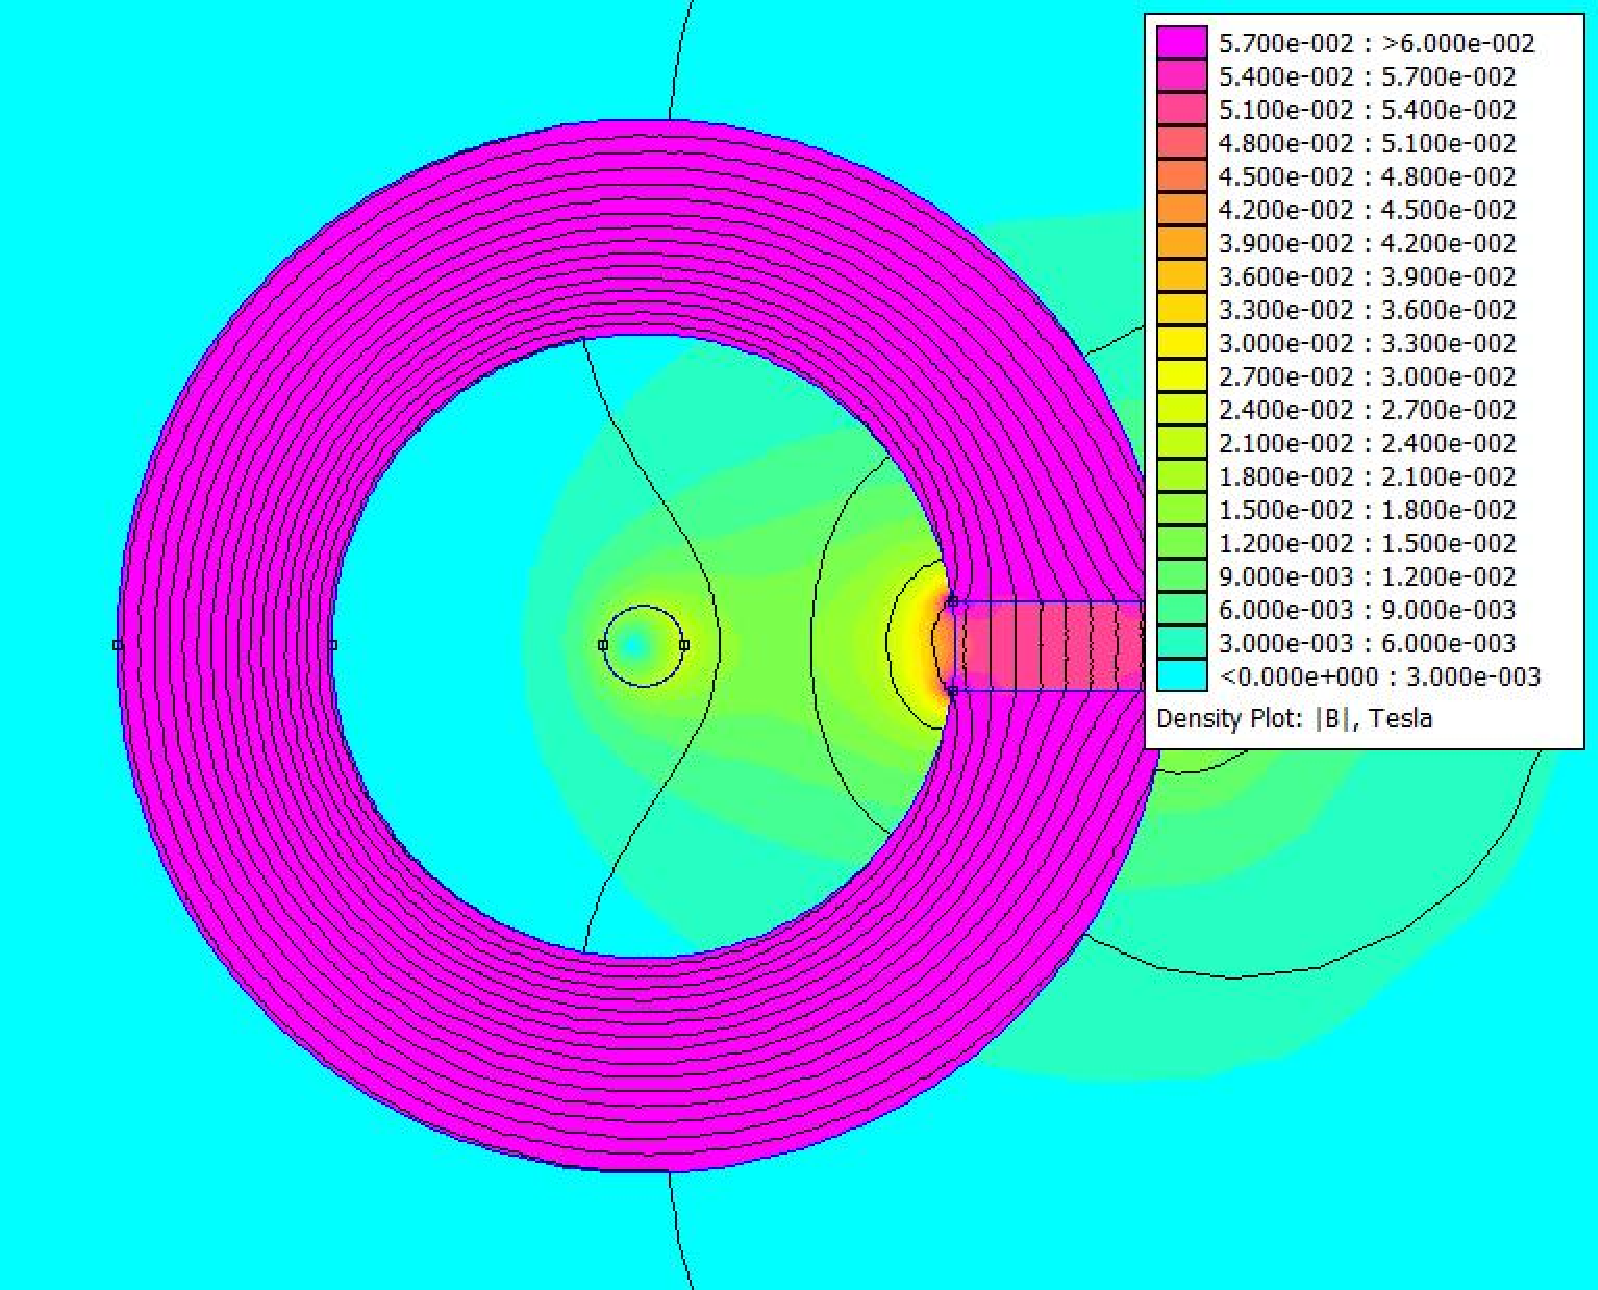
\includegraphics[width=0.7\textwidth]{single_gap.pdf}
\caption{Densidade de fluxo magnético no sensor único isolado, a
\SI{100}{\ampere}. O entreferro (região clara à direita do núcleo)
concentra o campo no ponto de medição do elemento Hall.}
\label{fig:single_gap}
{\small Fonte: Autor (2026), simulação FEMM.}
\end{figure}

A varredura de corrente da Configuração~1 (\SI{1}{\ampere} a
\SI{100}{\ampere}) confirma o comportamento linear assumido em
\autoref{sec:ganho_transferencia}: a densidade de fluxo no entreferro cresce
proporcionalmente à corrente (Figura~\ref{fig:I_vs_B}), e a sensibilidade
$G_{núcleo}$ permanece constante -- dentro da resolução numérica -- em toda
a faixa avaliada (Figura~\ref{fig:linearidade}).

\begin{figure}[h]
\centering
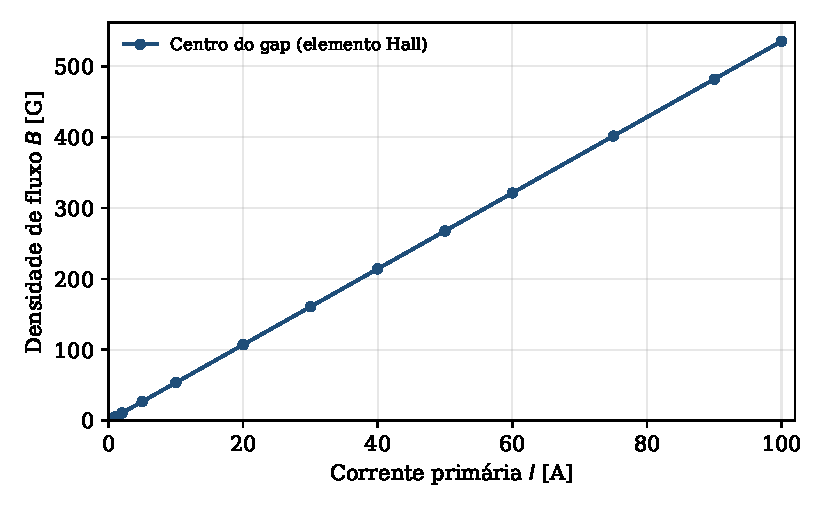
\includegraphics[width=0.75\textwidth]{fig_I_vs_B.pdf}
\caption{Densidade de fluxo no entreferro em função da corrente primária.}
\label{fig:I_vs_B}
{\small Fonte: Autor (2026).}
\end{figure}

\begin{figure}[h]
\centering
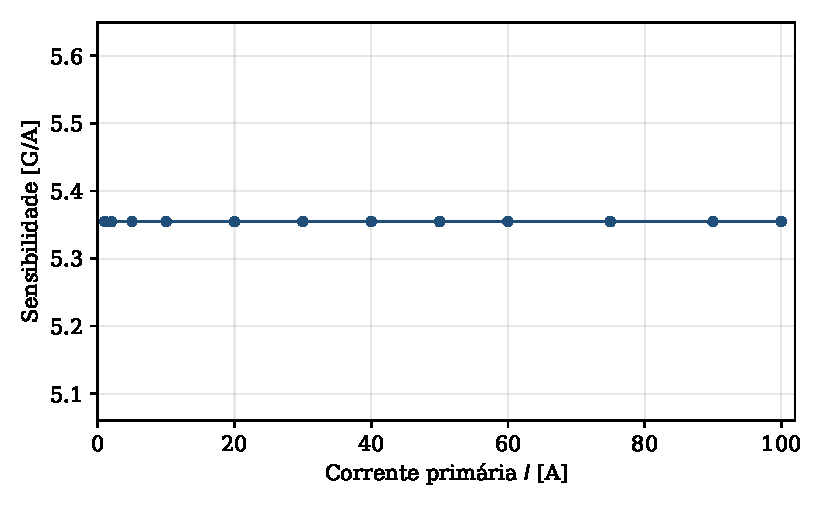
\includegraphics[width=0.75\textwidth]{fig_linearidade.pdf}
\caption{Sensibilidade $G_{núcleo}$ (G/A) em função da corrente primária --
uma curva horizontal indica comportamento linear.}
\label{fig:linearidade}
{\small Fonte: Autor (2026).}
\end{figure}

\begin{figure}[h]
\centering
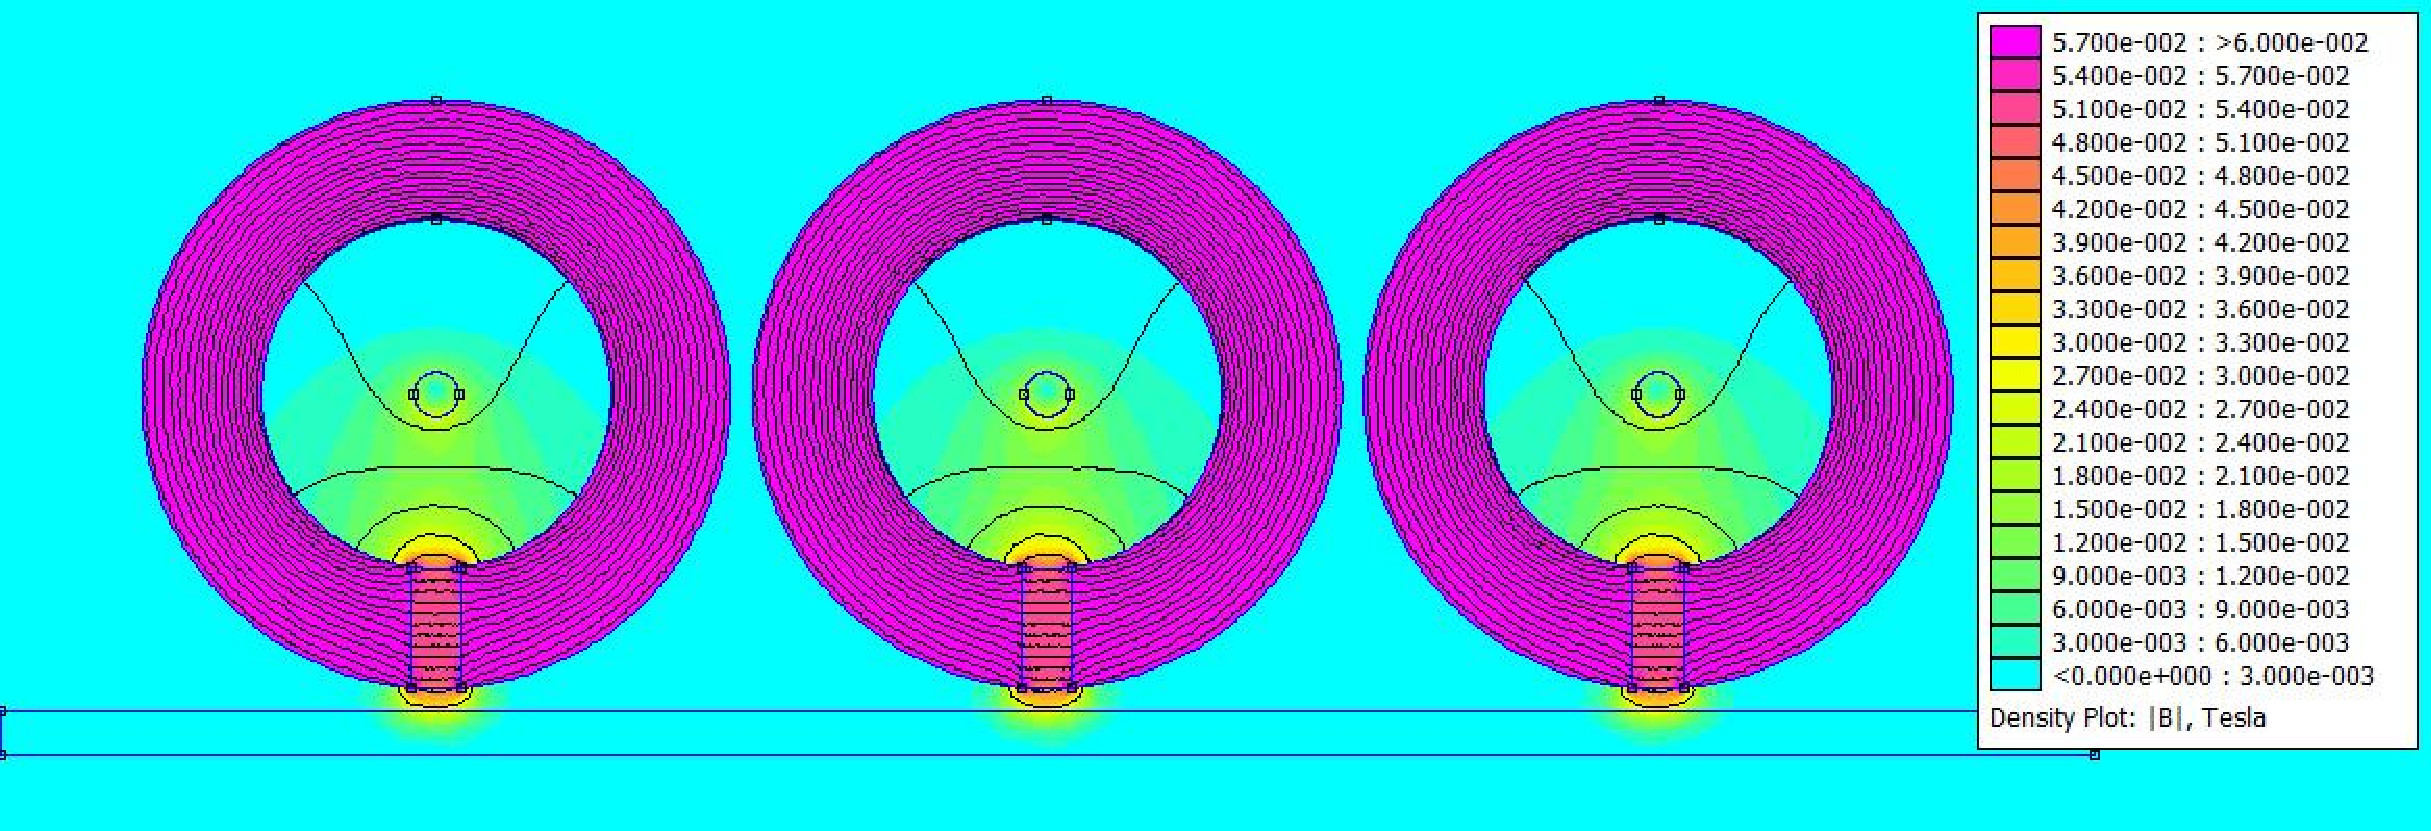
\includegraphics[width=\textwidth]{trifase_geral_d028mm.pdf}
\caption{Densidade de fluxo magnético nos três sensores de fase, três
condutores energizados simultaneamente a \SI{100}{\ampere}, menor distância
testada (\SI{28}{\milli\meter} entre centros). A faixa horizontal abaixo dos
núcleos é o plano de GND do PCB.}
\label{fig:trifase_geral}
{\small Fonte: Autor (2026), simulação FEMM.}
\end{figure}

Duas simplificações relevantes foram adotadas. O modelo planar (2D) ignora
o vazamento de fluxo pela altura do núcleo (\SI{12}{\milli\meter}), tratando
o resultado de ganho como um limite superior de referência, a confirmar por
medição direta em bancada. O ferrite foi modelado como material linear
($\mu_r$ constante, sem curva $B$--$H$), válido enquanto a densidade de
fluxo no núcleo permanecer abaixo do joelho de saturação -- confirmado pela
linearidade observada em toda a faixa de corrente simulada. A fronteira do
domínio de solução foi fechada pela condição de contorno assintótica
embutida do FEMM, dimensionada para envolver toda a geometria com folga.

\section{Acoplamento Entre Sensores Adjacentes (\textit{Crosstalk})}
\label{sec:crosstalk}

Para quantificar o acoplamento magnético entre sensores adjacentes, sete
combinações de correntes foram simuladas em cada distância avaliada: cada
fase isoladamente (\SI{100}{\ampere} em uma fase, demais em zero), cada par
de fases simultaneamente, e as três fases simultaneamente. A leitura de cada
sensor no cenário em que apenas sua própria fase está energizada serve de
referência ``sem interferência''; o desvio nos demais cenários quantifica o
\textit{crosstalk} introduzido pelos sensores vizinhos.

\begin{figure}[h]
\centering
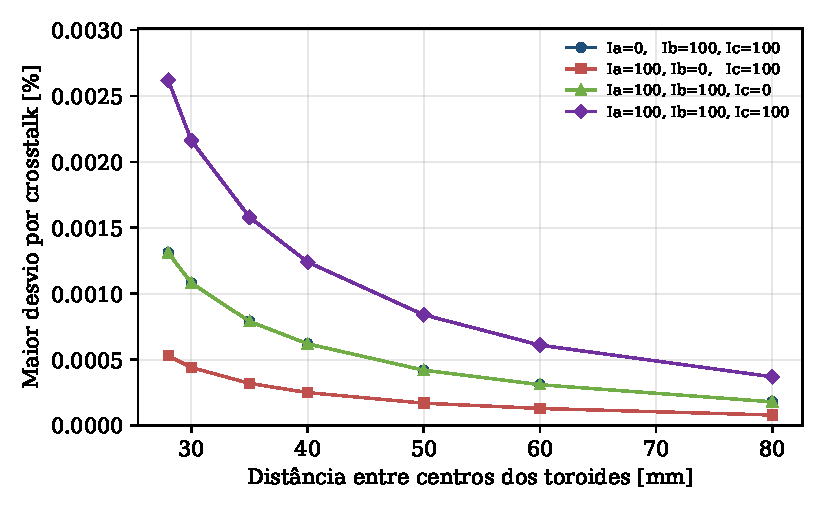
\includegraphics[width=0.85\textwidth]{fig_crosstalk.pdf}
\caption{Maior desvio de leitura por \textit{crosstalk} entre fases, em
função da distância entre centros dos núcleos, \SI{12}{\kilo\hertz}.}
\label{fig:crosstalk}
{\small Fonte: Autor (2026).}
\end{figure}

\begin{table}[h]
\centering
\caption{Maior desvio por \textit{crosstalk} em função da distância entre
centros dos núcleos (CA, \SI{12}{\kilo\hertz}).}
\label{tab:crosstalk_resumo}
\begin{tabular}{cc}
\toprule
\textbf{Distância entre centros} & \textbf{Maior desvio} \\
\midrule
\SI{28}{\milli\meter} & \SI{0,00262}{\percent} \\
\SI{30}{\milli\meter} & \SI{0,00216}{\percent} \\
\SI{35}{\milli\meter} & \SI{0,00158}{\percent} \\
\SI{40}{\milli\meter} & \SI{0,00124}{\percent} \\
\SI{50}{\milli\meter} & \SI{0,00084}{\percent} \\
\SI{60}{\milli\meter} & \SI{0,00061}{\percent} \\
\SI{80}{\milli\meter} & \SI{0,00037}{\percent} \\
\bottomrule
\end{tabular}

\vspace{2pt}
{\small Fonte: Autor (2026), simulação FEMM.}
\end{table}

O desvio máximo observado foi de \SI{0,0026}{\percent}, na menor distância
testada, decaindo monotonicamente com o afastamento entre núcleos
(Figura~\ref{fig:crosstalk} e Tabela~\ref{tab:crosstalk_resumo}). Mesmo no
pior caso -- núcleos no limite físico de proximidade --, o
\textit{crosstalk} está três ordens de grandeza abaixo de um limiar de
\SI{1}{\percent}, adotado como referência de desprezibilidade. A proximidade
entre os sensores de corrente das três fases, portanto, não compromete a
precisão da medição individual de cada fase em nenhum espaçamento
fisicamente viável de PCB.

\section{Acoplamento Indutivo Parasita}
\label{sec:acoplamento_indutivo}

Além do acoplamento de campo na leitura (\textit{crosstalk},
\autoref{sec:crosstalk}), avaliou-se se a introdução dos três núcleos e do
plano de GND perturba a própria dinâmica elétrica do acionamento,
modelando cada condutor de fase -- com seu núcleo e vizinhança -- como um
indutor acoplado aos demais, conforme a Figura~\ref{fig:indutores_acoplados}.
A indutância própria de cada fase ($L_{AA}$, $L_{BB}$, $L_{CC}$) e a
indutância mútua entre pares ($M_{AB}$, $M_{AC}$, $M_{BC}$) foram extraídas
do enlace de fluxo de cada circuito, já calculado pelo FEMM durante a
resolução do campo -- sem simulações adicionais.

\begin{figure}[h]
\centering
\begin{tikzpicture}[
    decoration={coil, aspect=0.5, segment length=3.2pt, amplitude=2.6pt},
    >=Latex,
    font=\small
]
    % tres indutores (fases A, B, C)
    \draw[decorate] (0,0) -- (2.2,0);
    \draw[decorate] (3.6,0) -- (5.8,0);
    \draw[decorate] (7.2,0) -- (9.4,0);

    \node[below] at (1.1,-0.05) {$L_{AA}$};
    \node[below] at (4.7,-0.05) {$L_{BB}$};
    \node[below] at (8.3,-0.05) {$L_{CC}$};
    \node[below, yshift=-12pt] at (1.1,-0.05) {\footnotesize$\approx\SI{59,3}{\nano\henry}$};
    \node[below, yshift=-12pt] at (4.7,-0.05) {\footnotesize$\approx\SI{59,3}{\nano\henry}$};
    \node[below, yshift=-12pt] at (8.3,-0.05) {\footnotesize$\approx\SI{59,3}{\nano\henry}$};

    \node[above] at (-0.3,0) {Fase $A$};
    \node[above] at (3.3,0) {Fase $B$};
    \node[above] at (6.9,0) {Fase $C$};

    % acoplamentos mutuos -- arcos com seta dupla
    \draw[<->, thick] (1.1,0.55) to[bend left=35] node[above, yshift=1pt] {$M_{AB}$} (4.7,0.55);
    \draw[<->, thick] (4.7,0.55) to[bend left=35] node[above, yshift=1pt] {$M_{BC}$} (8.3,0.55);
    \draw[<->, thick] (1.1,1.55) to[bend left=18] node[above, yshift=1pt] {$M_{AC}$} (8.3,1.55);

    \node[align=center, font=\footnotesize] at (2.9,0.95) {$\approx\SI{0,72}{\pico\henry}$};
    \node[align=center, font=\footnotesize] at (6.5,0.95) {$\approx\SI{0,72}{\pico\henry}$};
    \node[align=center, font=\footnotesize] at (4.7,2.05) {$\approx\SI{0,29}{\pico\henry}$};

    % distancia entre centros
    \draw[<->] (1.1,-0.9) -- node[below] {$d$} (4.7,-0.9);
    \draw[<->] (4.7,-0.9) -- node[below] {$d$} (8.3,-0.9);
\end{tikzpicture}
\caption{Modelo de indutores acoplados das três fases: indutância própria
$L$ de cada núcleo e indutância mútua $M$ entre pares, com valores extraídos
da simulação para $d=\SI{28}{\milli\meter}$ (menor distância testada).}
\label{fig:indutores_acoplados}
{\small Fonte: Autor (2026).}
\end{figure}

A Tabela~\ref{tab:inducao_resumo} apresenta os valores extraídos nos dois
extremos da varredura de distância, incluindo o coeficiente de acoplamento
$k_{xy} = M_{xy}/\sqrt{L_{xx}L_{yy}}$, que normaliza a mútua pelas próprias
indutâncias e é diretamente comparável ao $k$ usado para transformadores e
indutores acoplados convencionais ($k=1$ representa acoplamento perfeito).

\begin{table}[h]
\centering
\caption{Indutância própria, mútua e coeficiente de acoplamento nos extremos
da varredura de distância (CA, \SI{12}{\kilo\hertz}).}
\label{tab:inducao_resumo}
\begin{tabular}{lcc}
\toprule
\textbf{Grandeza} & \textbf{$d=\SI{28}{\milli\meter}$} & \textbf{$d=\SI{80}{\milli\meter}$} \\
\midrule
$L_{AA}$, $L_{BB}$, $L_{CC}$ & $\approx\SI{59,3}{\nano\henry}$ & $\approx\SI{59,3}{\nano\henry}$ \\
$M_{AB}$, $M_{BC}$ (adjacentes) & \SI{0,723}{\pico\henry} & \SI{0,102}{\pico\henry} \\
$M_{AC}$ (extremos) & \SI{0,292}{\pico\henry} & \SI{0,041}{\pico\henry} \\
$k_{AB}$, $k_{BC}$ & \num{1.22e-5} & \num{1.72e-6} \\
$k_{AC}$ & \num{4.92e-6} & \num{6.98e-7} \\
\bottomrule
\end{tabular}

\vspace{2pt}
{\small Fonte: Autor (2026), simulação FEMM.}
\end{table}

\begin{figure}[h]
\centering
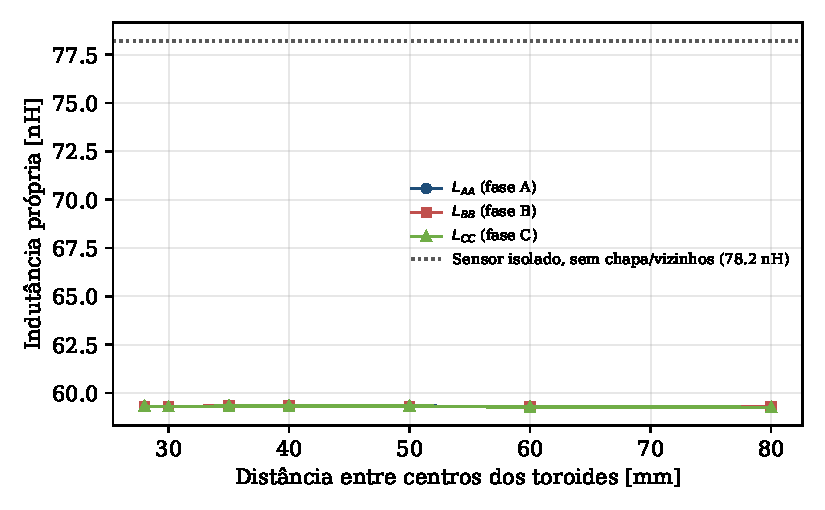
\includegraphics[width=0.85\textwidth]{fig_inductancia_self.pdf}
\caption{Indutância própria de cada fase em função da distância entre
centros, com referência tracejada do núcleo isolado (sem chapa/vizinhos).}
\label{fig:inductancia_self}
{\small Fonte: Autor (2026).}
\end{figure}

\begin{figure}[h]
\centering
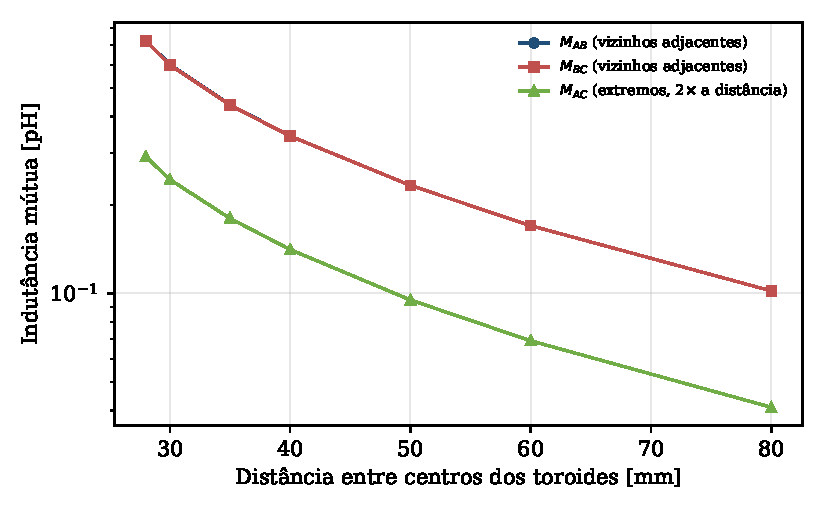
\includegraphics[width=0.85\textwidth]{fig_inductancia_mutua.pdf}
\caption{Indutância mútua entre pares de fases em função da distância entre
centros (escala logarítmica).}
\label{fig:inductancia_mutua}
{\small Fonte: Autor (2026).}
\end{figure}

\begin{figure}[h]
\centering
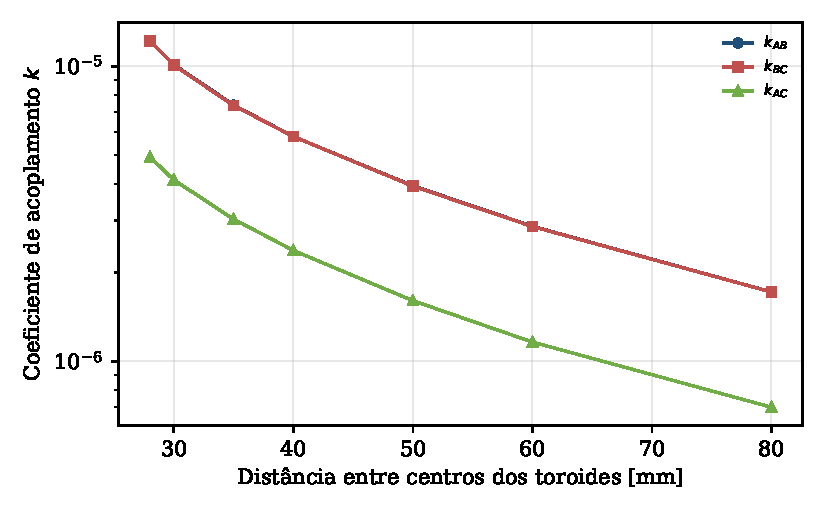
\includegraphics[width=0.85\textwidth]{fig_coef_acoplamento.pdf}
\caption{Coeficiente de acoplamento $k=M/\sqrt{L_xL_y}$ entre pares de fases
em função da distância entre centros (escala logarítmica).}
\label{fig:coef_acoplamento}
{\small Fonte: Autor (2026).}
\end{figure}

A indutância própria (Figura~\ref{fig:inductancia_self}) mantém-se
praticamente constante ao longo de toda a varredura de distância -- esperado,
já que a geometria de cada sensor com a placa de GND não muda com o
espaçamento entre sensores, apenas a distância \emph{entre} eles.
Notavelmente, esse valor ($\approx\SI{59,3}{\nano\henry}$) é \emph{menor}
que a indutância própria de um núcleo isolado, sem chapa nem vizinhos
(\SI{78,3}{\nano\henry} em CC, \SI{78,2}{\nano\henry} em
\SI{12}{\kilo\hertz}): a proximidade do plano de cobre reduz a indutância
própria em cerca de \SI{24}{\percent}, um efeito de plano-imagem causado
pelas correntes de Foucault induzidas na placa, que se opõem à penetração do
fluxo -- efeito real e mensurável, ainda que de magnitude irrelevante frente
à indutância de fase típica de um acionamento trifásico (tipicamente dezenas
de \si{\micro\henry} a poucos \si{\milli\henry}).

A indutância mútua (Figura~\ref{fig:inductancia_mutua}) decai de
aproximadamente \SI{0,72}{\pico\henry} entre fases adjacentes na menor
distância testada até \SI{0,10}{\pico\henry} em \SI{80}{\milli\meter}; o par
de fases nos extremos do arranjo apresenta consistentemente cerca da metade
do acoplamento dos pares adjacentes. O coeficiente de acoplamento
(Figura~\ref{fig:coef_acoplamento}) varia entre $k\approx\num{1.2e-5}$ e
$k\approx\num{7e-7}$ -- ordens de grandeza abaixo de qualquer acoplamento
indutivo relevante. Como verificação de consistência, a indutância mútua foi
calculada de duas formas independentes para cada par (energizando cada fase
separadamente); a maior divergência entre os dois cálculos foi de apenas
\SI{0,43}{\percent}, confirmando a qualidade da malha e da geometria.

Tanto a indutância própria adicionada (dezenas de \si{\nano\henry}) quanto o
acoplamento mútuo entre fases (frações de \si{\pico\henry}) são desprezíveis
frente à indutância de fase típica de acionamentos trifásicos de pequeno/médio
porte. Conclui-se que o arranjo de sensores de corrente proposto não deve
introduzir perturbação elétrica mensurável na dinâmica do acionamento, em
nenhuma das distâncias de montagem avaliadas.

\end{document}
